\documentclass[]{elsarticle} %review=doublespace preprint=single 5p=2 column
%%% Begin My package additions %%%%%%%%%%%%%%%%%%%
\usepackage[hyphens]{url}
\usepackage{lineno} % add
\providecommand{\tightlist}{%
  \setlength{\itemsep}{0pt}\setlength{\parskip}{0pt}}

\bibliographystyle{elsarticle-harv}
\biboptions{sort&compress} % For natbib
\usepackage{graphicx}
\usepackage{booktabs} % book-quality tables
%% Redefines the elsarticle footer
%\makeatletter
%\def\ps@pprintTitle{%
% \let\@oddhead\@empty
% \let\@evenhead\@empty
% \def\@oddfoot{\it \hfill\today}%
% \let\@evenfoot\@oddfoot}
%\makeatother

% A modified page layout
\textwidth 6.75in
\oddsidemargin -0.15in
\evensidemargin -0.15in
\textheight 9in
\topmargin -0.5in
%%%%%%%%%%%%%%%% end my additions to header

\usepackage[T1]{fontenc}
\usepackage{lmodern}
\usepackage{amssymb,amsmath}
\usepackage{ifxetex,ifluatex}
\usepackage{fixltx2e} % provides \textsubscript
% use upquote if available, for straight quotes in verbatim environments
\IfFileExists{upquote.sty}{\usepackage{upquote}}{}
\ifnum 0\ifxetex 1\fi\ifluatex 1\fi=0 % if pdftex
  \usepackage[utf8]{inputenc}
\else % if luatex or xelatex
  \usepackage{fontspec}
  \ifxetex
    \usepackage{xltxtra,xunicode}
  \fi
  \defaultfontfeatures{Mapping=tex-text,Scale=MatchLowercase}
  \newcommand{\euro}{€}
\fi
% use microtype if available
\IfFileExists{microtype.sty}{\usepackage{microtype}}{}
\usepackage{graphicx}
% We will generate all images so they have a width \maxwidth. This means
% that they will get their normal width if they fit onto the page, but
% are scaled down if they would overflow the margins.
\makeatletter
\def\maxwidth{\ifdim\Gin@nat@width>\linewidth\linewidth
\else\Gin@nat@width\fi}
\makeatother
\let\Oldincludegraphics\includegraphics
\renewcommand{\includegraphics}[1]{\Oldincludegraphics[width=\maxwidth]{#1}}
\ifxetex
  \usepackage[setpagesize=false, % page size defined by xetex
              unicode=false, % unicode breaks when used with xetex
              xetex]{hyperref}
\else
  \usepackage[unicode=true]{hyperref}
\fi
\hypersetup{breaklinks=true,
            bookmarks=true,
            pdfauthor={},
            pdftitle={Inter and Intra-Regional Spillovers of Global External-Competitiveness},
            colorlinks=true,
            urlcolor=blue,
            linkcolor=magenta,
            pdfborder={0 0 0}}
\urlstyle{same}  % don't use monospace font for urls
\setlength{\parindent}{0pt}
\setlength{\parskip}{6pt plus 2pt minus 1pt}
\setlength{\emergencystretch}{3em}  % prevent overfull lines
\setcounter{secnumdepth}{0}
% Pandoc toggle for numbering sections (defaults to be off)
\setcounter{secnumdepth}{0}
% Pandoc header


\usepackage[nomarkers]{endfloat}

\begin{document}
\begin{frontmatter}

  \title{Inter and Intra-Regional Spillovers of Global External-Competitiveness}
    \author[West Virginia University]{Shishir Shakya\corref{c1}}
   \ead{shishir.shakya@mail.wvu.edu} 
   \cortext[c1]{Corresponding Author}
    \author[West Virginia University]{Alexandre R. Scarcioffolo}
   \ead{alexandre.ribeiroscarcioffolo@mail.wvu.edu} 
  
      \address[West Virginia University]{College of Business and Economics \& Regional Research Institute (RRI),
West Virginia University}
    \address[Another University]{Davis College of Agriculture, Natural Resources and Design \& Regional
Research Institute (RRI), West Virginia University}
  
  \begin{abstract}
  The 2007 U.S. sub-prime mortgage crisis spillover globally in 2008,
  sharply affecting the entire world, especially European countries. Ever
  since, measuring and mapping how the shocks are transmitted and received
  in such global network has become a vital research domain. Several
  papers by Diebold and Yilmaz (2009, 2014, 2015) laid foundations to
  analyze the financial interrelatedness based on the stock prices.
  However, in this paper, we investigated the dynamics of connectedness of
  external-competitiveness by mapping how countries are economically
  connected to transmit and receive external-competitiveness and by
  ranking the economies based on their ability to transmit or receive
  external-competitiveness. In our study, the external-competitiveness
  refers to the nation's capability to trade at the competitive prices in
  the international economy. As the proxy for external competitiveness, we
  retrieved the daily data (10/3/1983 - 2/14/2017) of effective exchange
  rate (EER ) from the Bank of International Settlements (BIS) for 25
  major economies which includes Group of Ten (G10) , along with,
  Australia, Austria, Denmark, Finland, Greece, Ireland, New Zealand,
  Norway, Portugal and Spain and the four ``Asian Newly Industrialized
  Economies'' (NIE's).
  \end{abstract}
  
 \end{frontmatter}

\section{Introduction}\label{introduction}

The intricately interconnectedness of global economies due to
deregulation, liberalization, and spatial specialization in production
followed by succession of revolutionary advances in information and
communications technologies, in one hand have promoted economic
prosperity while in other, have made economys vulnerable to shocks
regardless of the origin of the shocks (Park and Shin 2017). Foreseeing
how events in one country or region might spillover to other countries
is primordial to Governments, private companies, and private investors.
By doing so, Government's leaders can anticipate disruptive global
shocks by incentive their own economy as well as by protecting vital
sectors that might be essential to the nation, guaranteeing the welfare
while improving the economic performance during a distress moment.
Moreover, global private companies can efficiently change corporate
investment in regions/sectors that might be heavily affected to
investments that do not bring that level of uncertainty. Finally,
through the lens of private investors, having better information
regarding the global economy conditions might improve the allocation of
their portfolios, maximizing gains through arbitrage. Therefore,
measuring and mapping how economic shocks are transmitted and received
in such global network has become a vital research domain in which this
study focus on understudying the dynamics of countries' competitiveness
with respect to global economic shocks.

Periods of distress economies such as the European Monetary System (EMS)
crisis 1992-1993, the Mexican crisis (Tequila crisis) in the end of
1994; the Thailand crisis (Asian flu) in 1997; Russian crisis (Russian
virus) in 1998 and the Argentinean crisis in 2001 have persistently
proven the financial and economic turbulence as the ramifications of
interconnected world (Kali and Reyes 2010). Further, the 2007 U.S.
sub-prime mortgage crisis followed by Lehman Brothers collapse spillover
globally in 2008 sharply affecting the world and triggering the European
debt crisis in 2009. Voluminous researches have concentrated on the
connectedness of financial markets and its interactions while (see F. X.
Diebold and Yilmaz 2009, F. X. Diebold and Yilmaz (2012), F. X. Diebold
and Yilmaz (2013), F. X. Diebold and Yilmaz (2014), Barunik and Krehlik
(2015), F. X. Diebold and Yilmaz (2015)) are pioneers.

Although, due to high linked and globalized world in which shocks move
regardless of geographic boundaries, identifying the transmiter and
receiver of shocks can be applied to broader contexts. For an example:
F. X. Diebold and Yilmaz (2013) examine business cycle connectedness of
U.S.A, Japan, France, Germany, U.K. and Italy; Awartani, Aktham, and
Cherif (2016) investigate the directional risk transfer from oil to US
equities, Euro/Dollar exchange rates, precious metals and agricultural
commodities and Barunik and Krehlik (2015) used rich time-frequency
dynamics of volatility connectedness in US financial institutions;
Billio et al. (2012) measure the connectedness of returns of hedge
funds, banks, broker/dealers, and insurance companies based on principal
components analysis and Granger causality networks; Bubák, Kočenda, and
Žikeš (2011) study the dynamics of volatility transmission between
Central European (CE) currencies and the EUR/USD foreign exchange;
Cimini (2015) 80 largest eurozone financial and non-financial entities
in terms of market capitalisation. \textbf{I will cite trade networks,
sectorial networks and financial too and we will seggregate..}

One area of interest that is underrate and quite controversial is to
measure the dynamics of international competitiveness. In general, the
concept of ``competitiveness'' can conclave the multidimensional facets
of market performances that relates to product quality, ability to
innovate, rapidly adjust to customer needs, and absence of the
restrictive practice in labor market (Turner and Van'tdack 1993).
Nonetheless, its interpretation can be easily misleading since there is
no unique definition of the term ``competitiveness''. According to
Krugman (1994), the word ``competitiveness'' has two different meaning
depends on its application. Corporation competitiveness, it is a
zero-sum game, of which if a firm A is losing its competitiveness
(market share), other firms will incorporate it until the firm A goes
bankrupt. On the other hand, when we refer to competitiveness in a
international perspective, we cannot use the same definition above since
countries do not go out of business. Hence, international
competitiveness being one area of interest is controversial and thus
measurement of the dynamics of international competitiveness can suffer
the definitional sensitivities. But within these definitional hurdles of
international competitiveness, in one hand, its clear that relative cost
or prices if are too high can deter to compete internationally.
Meanwhile, this clarity on the concept of competitiveness tend to be
very ``Zen'' like because, in other hand, strong economic performances
appreciates the exchange rate thus leads to higher relative cost.

Turner and Van'tdack (1993) clarify that if enterprises in a country
become more successful in the non-price dimensions of performance- if
they are innovative, flexible, produce high-quality goods and so on
-then the real exchange rate would be expected to strengthen. Price and
wage competitiveness -the narrow concept- would thus appear to
``worsen''. But such ``deterioration'' would of course be a symptom of
success, not of failure. For the narrow concept, the effective exchange
rates can be a proxy for the short run price competitiveness.

Even though our paper is mainly centers around the narrower concept of
competitiveness. But translating this perception into operation measures
has always faced formidable difficulties. Many attempts have been seen
to quantify the price or cost competitiveness using the Real Effective
Exchange rates. Fed, EU, JP, BIS..the trend appears about the same.
However, we take a special precaution to interpret the Effective
exchange rate.

The concept of effective exchange rate was formalized after the
breakdown of the multilateral Bretton Woods system of pegged but
adjustable exchange rates in the early 1970s. Since, currencies have
entered a new era of non-orderly floating exchange rates, leaving it at
countries- discretion to choose their particular exchange rate regime.
Members of today's European Union established a new regional system of
pegged but adjustable exchange rates, and at the end of the 1990s, some
of them permanently fixed their exchange rates and adopted the euro as
their common currency. Among developing countries, too, many have chosen
to peg their currencies to or stabilize them against some anchor
currencies, most prominently the United States dollar, at least during
some of the time (UNCTAD 2012).

EER is the trade-weighted average exchange rate of a currency against a
basket of currencies and the EER adjusted for inflation gives real EER
(REER). In both policy and market analysis, EERs serve various purposes:
as a measure of international competitiveness, as components of
monetary/financial conditions indices, as a gauge of the transmission of
external shocks, as an intermediate target for monetary policy or as an
operational target (Klau and Fung 2006).

However, the controversy persists even in this narrow concept mainly
because of distinct statistical from of cost and prices indices and
their relativity. If we discuss about relativity (to whom or which
country to compare with and by how much and at which time or base year)
it again varies upon the choices of currency basket, their weights and
base year, while, we discuss about the price or cost measure for the
industrial countries, the competitiveness depends upon the unit of labor
costs (mostly in manufacturing ), consumer price or other broadly-based
price index and the export unit values. A comprehensive survey of all
the issues related to measuring effective exchange rate in given in
(Koch 1984).

To create choices of currencies basket the currency should be at least
convertibility or exchangeable at multiple exchange rate and the nature
of inflation of the countries should have moderate inflation. Because,
incorporating high inflation currencies in the index calculation would
mean that nominal indexes over time become dominated by the rapidly
declining external value of inflation-prone currencies.

While the currencies weights are derived with various weighting schemes
like: general equilibrium model-based weights like the Multilateral
Exchange Rate Model (MERM) of the IMF and trade-weighting schemes based
on the bilateral trade flows, global trade flows and double weights. The
bilateral or global trade flows are essentially special cases of the
double-weighting scheme. In a bilateral scheme it is implicitly assumed
that in each export market the domestic producer constitutes the sole
competitor, completely ruling out competition from other exporters to
that market (i.e.~competition in ``third markets''). Only in each
country's home market is competition between various foreign suppliers
allowed for. This weighting scheme thus assigns weights to trading
partners strictly in proportion to their share in the home country's
exports and imports. Finally, under a global scheme it is assumed that
all individual country markets collapse into a single world market in
which only exporters compete. Under this assumption the currencies of
partner countries are weighted in proportion to their share in world
trade.

While few other papers test the co-movement of real effective exchange
rate (Nagayasu 2017), these studies are rather limited as they do not
report the direction of the shocks between countries, and also do not
specify the relative magnitudes of their contributions. Thus, this gives
us that there is a potential ground of improvement by , analyzing to the
dynamics of analyze the inter and intra-regional analysis of
competitiveness. Therefore, the purposes of the present paper are to
investigate the dynamics of connectedness of external-competitiveness by
mapping how countries are economically connected to transmit and receive
price-competitiveness and by ranking the economies based on their
ability to transmit or receive price-competitiveness. As the proxy for
price-competitiveness,
\textcolor{red}{Shishir will change this after defining the sample}we
retrieved the daily data (10/3/1983 - 2/14/2017) of effective exchange
rate (EER) from the Bank of International Settlements (BIS) for 25 major
economies which includes Group of Ten (G10) , along with, Australia,
Austria, Denmark, Finland, Greece, Ireland, New Zealand, Norway,
Portugal and Spain and the four ``Asian Newly Industrialized Economies''
(NIE's) . Also, to assess the time-varying global competitiveness, we
also perform the analysis in fixed period rolling window methodology.

Instead of using the data of the asset prices or exchange rates
\textbf{( \textcolor{red}{Needs citations}which many other researchers
use)} we use the data of effective exchange rate.
\textbf{\textcolor{red}{Needs citations}}The Dornbusch model or
overshooting theory provides a theoretical foundation that the financial
market and exchange rate markets over-react promptly on unanticipated
policy/shock, while, goods markets equilibrate gradually and over the
time, exuberating financial and exchange rate markets dissipates.

For an example, on December 17 of 2014, President of United States of
America, announced to normalize the relation to Cuba
\textbf{\textcolor{red}{Needs citations}}, and within two days, the
Herzfeld Caribbean Basin Fund Inc.- A closed end fund management
company- which has ``CUBA'' as the ticker symbol and has no exciting
company announcement, suddenly sells for a 70 percent higher premium
then gradually it reverts to its average past values
\textbf{\textcolor{red}{Needs citations}}. Hence, the study of financial
and exchange rate market potentially feedbacks false alarms. The
following graph shows such false alarm.

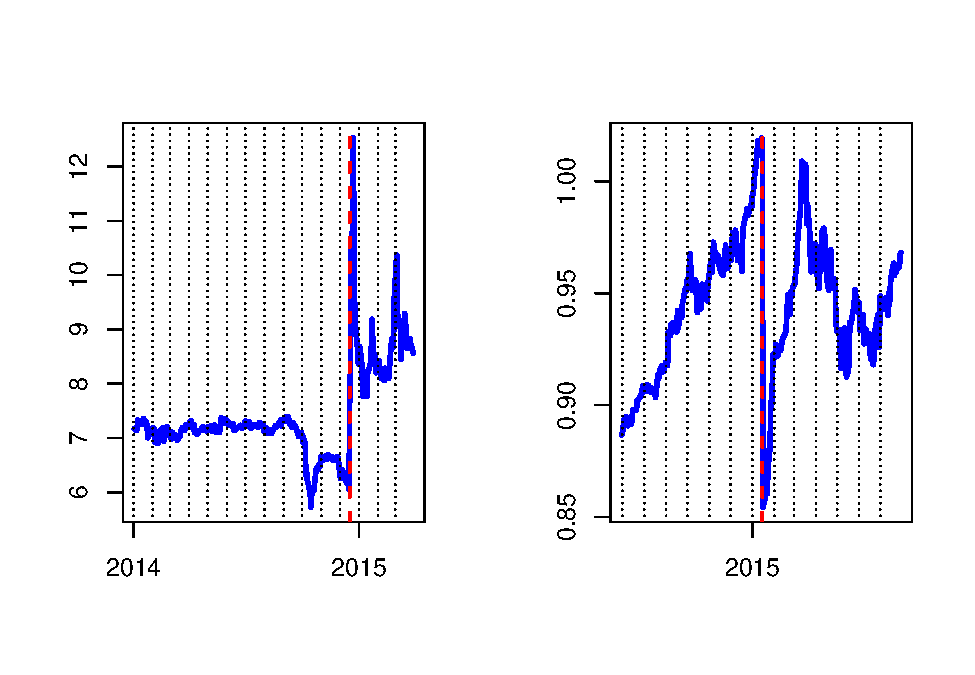
\includegraphics{Main_files/figure-latex/unnamed-chunk-1-1.pdf}

\section{Literature reviews}\label{literature-reviews}

\section{Data and methodologies}\label{data-and-methodologies}

\subsection{\texorpdfstring{\textbf{Data}}{Data}}\label{data}

Bank of International Settlement (BIS) defines two types of EER indexes
(EER): Broad and narrow. The broad EER consists of 61 advanced and
developing economies, whereas the narrow EER considers only 25 advanced
economies. Although the broad basket is more representative than the
narrow, neither should be regarded as the better measurement. The narrow
indices may better gauge the competitiveness among advanced countries
because their products have similar elasticities of substitution. The
broad indices, on the other hand, give a more global picture by taking
the emerging market economies into account. As a result, they would be
more useful in analyses of issues such as the sustainability of the
external trade balances. Our study is based on the broad EERs.

We retrieve broad nominal (available daily and monthly) and broad real
(available monthly) effective exchange rate (EER) index data available
from BIS for France, Germany, Italy, Japan, United Kingdom and United
States from 1996-04-08 to 2018-02-26. These indices are base to 100 for
year 2010. We deflate daily nominal EER by respective monthly deflator
-which is ratio of monthly nominal and real effective exchange rate- to
generate daily real EER (REER).

For the analysis, we developed two sets of data. First, we consider the
are the growth rates of the weekly REER of each economy (see Figure 1)
and second is the weekly volatility index (see Figure 2) based on the
daily REER under the assumption of the volatility is fixed within the
weekly period but variable across weeks following Garman, Mark and Klass
(1980) and Alizadeh, Brandt, and Diebold (2002) methodology. We consider
the REER of Monday and Friday as weekly opening and closing value, and
weekly minimum and maximum as the low and close value. The weekly
estimated volatility is calculate as following:

\[{{\hat{\sigma }}^{2}}=0.511{{\left( {{H}_{t}}-{{L}_{t}} \right)}^{2}}-0.019\left[ \left( {{C}_{t}}-{{O}_{t}} \right)\left( {{H}_{t}}+{{L}_{t}}-2{{O}_{t}} \right)-2\left( {{H}_{t}}-{{O}_{t}} \right)\left( {{L}_{t}}-{{O}_{t}} \right) \right]-0.383{{\left( {{C}_{t}}-{{O}_{t}} \right)}^{2}}\]

where, \(H\) is the Monday-Friday high, \(L\) is the Monday-Friday low,
\(O\) is the Monday open and \(C\) is the Friday close (all in natural
logarithms).

\subsubsection{\texorpdfstring{\textbf{Figure 1: Trend of weekly real
effective exchange rate from 1996-04-08 to
2018-02-26.}}{Figure 1: Trend of weekly real effective exchange rate from 1996-04-08 to 2018-02-26.}}\label{figure-1-trend-of-weekly-real-effective-exchange-rate-from-1996-04-08-to-2018-02-26.}

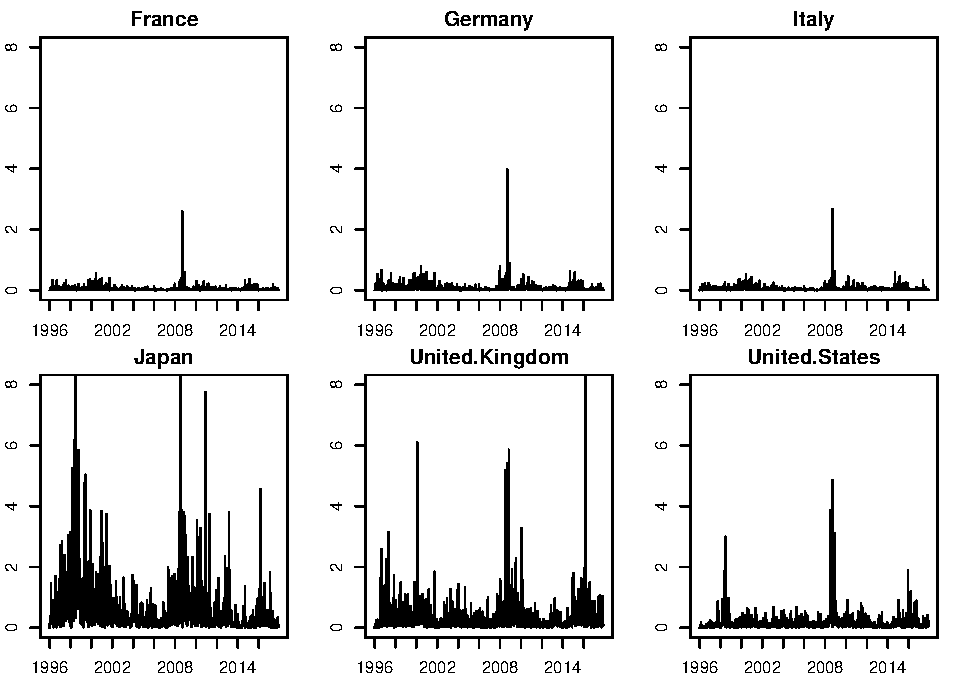
\includegraphics{Main_files/figure-latex/unnamed-chunk-4-1.pdf}

\subsubsection{\texorpdfstring{\textbf{Figure 2: Volatility of weekly
real effective exchange rate from 1996-04-08 to
2018-02-26.}}{Figure 2: Volatility of weekly real effective exchange rate from 1996-04-08 to 2018-02-26.}}\label{figure-2-volatility-of-weekly-real-effective-exchange-rate-from-1996-04-08-to-2018-02-26.}

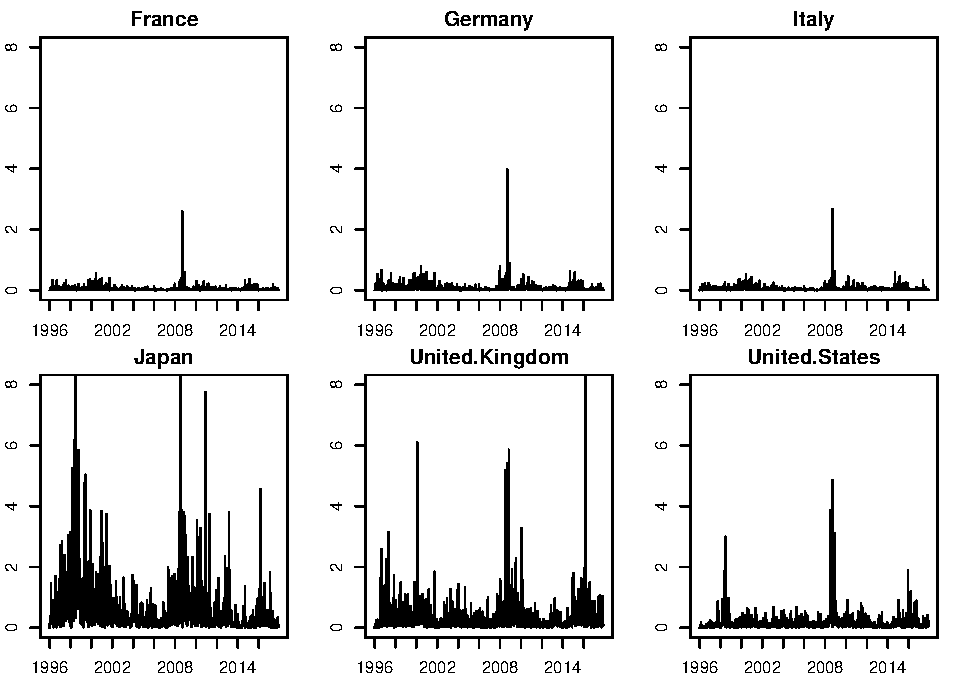
\includegraphics{Main_files/figure-latex/unnamed-chunk-5-1.pdf}

\subsection{\texorpdfstring{\textbf{Diebold and Yilmaz
methodology}}{Diebold and Yilmaz methodology}}\label{diebold-and-yilmaz-methodology}

\subsubsection{\texorpdfstring{\textbf{Vector autoregression (VAR)
model}}{Vector autoregression (VAR) model}}\label{vector-autoregression-var-model}

Vector autoregression (VAR) model is a stochastic process to capture the
linear interdependencies among multiple stationary time series by
incorporating own lagged values, the lagged values of the other model
variables, and an error term. VAR modeling does not require as much
knowledge about the forces influencing a variable as do structural
models with simultaneous equations: The only prior knowledge required is
a list of variables which can be hypothesized to affect each other
intertemporally. Following Sims (1980), given \(N\) stationary
variables, a \(p\) lagged vector autoregression \(VAR\left( p \right)\)
system can be defined as:

\[{{x}_{t}}=\sum\nolimits_{i=1}^{p}{{{\Phi }_{i}}{{x}_{t-i}}+{{\varepsilon }_{t}}}\]

The basic component of Diebold and Yilmaz (D\&Y) model is the
generalized variance decomposition of forecast errors of an \(N-\)
variables (economies), \(p\) lagged covariance stationary vector
auto-regression \(VAR\left( p \right)\) approximating model. Such
\(VAR\left( p \right)\) system is defined as:

\[{{x}_{t}}=\sum\nolimits_{i=1}^{p}{{{\Phi }_{i}}{{x}_{t-i}}+{{\varepsilon }_{t}}}\]

where \({{\varepsilon }_{t}}\) is the vectors independently and
identically distributed disturbances and \(\Omega\) is the covariance
matrix. For a covariance stationary \(VAR\left( p \right)\) process
there exist the moving averages representation as
\({{x}_{t}}=\sum\nolimits_{i=0}^{\infty }{{{A}_{i}}{{\varepsilon }_{t-i}}}\),
where the \(N\times N\) coefficient matrix \({{A}_{i}}\) obey the
recursion
\({{A}_{i}}={{\Phi }_{1}}{{A}_{i-1}}+{{\Phi }_{2}}{{A}_{i-2}}+\cdots +{{\Phi }_{p}}{{A}_{i-p}}\)
with \({{A}_{0}}\) an \(N\times N\) identity matrix and \({{A}_{i}}=0\)
for \(i<0\).The moving averages coefficients (or transformations such as
impulse response functions or variance decomposition) provides the
dynamics of the system.

where, \({{\varepsilon }_{t}}\) is the vectors independently and
identically distributed disturbances and \(\Omega\) is the covariance
matrix. For a covariance stationary \(VAR\left( p \right)\) process
there exist the moving averages representation as
\({{x}_{t}}=\sum\nolimits_{i=0}^{\infty }{{{A}_{i}}{{\varepsilon }_{t-i}}}\),
where the \(N\times N\) coefficient matrix \({{A}_{i}}\) obey the
recursion
\({{A}_{i}}={{\Phi }_{1}}{{A}_{i-1}}+{{\Phi }_{2}}{{A}_{i-2}}+\cdots +{{\Phi }_{p}}{{A}_{i-p}}\)
with \({{A}_{0}}\) being an \(N\times N\) identity matrix and
\({{A}_{i}}=0\) for \(i<0\). The moving averages coefficients (or
transformations such as impulse response functions or variance
decomposition) provides the dynamics of the system.

\subsubsection{\texorpdfstring{\textbf{Variance decomposition matrix
(VDM) and various
connectedness}}{Variance decomposition matrix (VDM) and various connectedness}}\label{variance-decomposition-matrix-vdm-and-various-connectedness}

The variance decompositions allow to split the \(H\)-step ahead forecast
error of each variable into parts that can be attributable to the
various market shocks. The aggregation of these decompositions will be
subsequently used to compute the directional connectedness from an
economy to any or to all the included economy.

The variance decompositions computation is usually done by using
orthogonal VAR shocks. The Cholesky identification scheme achieves
orthogonality but the computed variance decompositions are then unstable
and they are dependent on the ordering of the marketsmodel. Thus,
Cholesky decomposition is not suitable. A framework that produces
order-invariant decompositions is the generalized variance
decompositions, of which it VAR that allows for correlated shocks but
accounts for them appropriately. The framework, which we denote KPPS,
has been first proposed by Koop et al. (1996) and Pesaran and Shin
(1998). The KPPS forecast error variance decomposition matrix (VDM) for
\(H\)-step ahead is computed as:

\[\theta _{ij}^{g}\left( H \right)=\frac{\sigma _{jj}^{-1}\sum\nolimits_{h=0}^{H-1}{{{\left( {{{{e}'}}_{i}}{{h}_{h}}\Omega {{e}_{j}} \right)}^{2}}}}{\sum\nolimits_{h=0}^{H-1}{\left( {{{{e}'}}_{i}}{{h}_{h}}\Omega {{e}_{j}} \right)}}\]

Where, \({{\sigma }_{jj}}\) is the standard deviation of the error term
of the \({{j}^{th}}\) economy and \({{e}_{i}}\) is a selection vector
with one on the \({{i}^{th}}\) element and zero otherwise.

\subsubsection{\texorpdfstring{\textbf{Pairwise direction
connectedness}}{Pairwise direction connectedness}}\label{pairwise-direction-connectedness}

To provide the information about the relative importance of each random
innovation to the variables in the VAR (information relative to the size
of endogenous and exogenous shocks on a given economy), we can normalize
each entry with its respective row as:

\[\tilde{\theta }_{ij}^{g}\left( H \right)=\frac{\theta _{ij}^{g}\left( H \right)}{\sum\nolimits_{j=1}^{N}{\theta _{ij}^{g}\left( H \right)}}\]

Which implies the row sum for any \({{i}^{th}}\) economy to be
\(\sum\nolimits_{j=1}^{N}{\tilde{\theta }_{ij}^{g}\left( H \right)}=1\),
hence row sums across all the economy be
\(\sum\nolimits_{i=1}^{N}{\sum\nolimits_{j=1}^{N}{\tilde{\theta }_{ij}^{g}\left( H \right)}}=N\).

Now each element of the row wise standardized VDM i.e
\({\tilde \theta _{ij}^g\left( H \right)}\) can be interpreted as the
pairwise directional connectedness from economy \(j\) to economy \(i\)
at horizon \(H\). For the intuitive purpose,
\({{C}_{i\leftarrow j}}\left( H \right)\) represents the pairwise
connectedness from economy \(j\) to economy \(i\) at horizon \(H\) and
the opposite direction pairwise connectedness from economy as
\({{C}_{j\leftarrow i}}\left( H \right)\). The net pairwise directional
connectedness then can be defined as

\[{{C}_{ij}}={{C}_{i\leftarrow j}}\left( H \right)-{{C}_{j\leftarrow i}}\left( H \right)\]

\subsubsection{\texorpdfstring{\textbf{Net-pairwise directional
connectedness}}{Net-pairwise directional connectedness}}\label{net-pairwise-directional-connectedness}

The net pairwise directional connectedness identifies the dominant
economy who transmit the information. Note that
\({{C}_{ij}}=-{{C}_{ji}}\) and if \({{C}_{ij}}>0\) then, economy
\(j\)transmit the information to economy \(i\).

To find how all the economy are jointly contributing to a single
economy, then the partial aggregation of connectedness from all economy
to economy \(i\) except from itself can be denoted as the row sum

\[{{C}_{i\leftarrow \bullet }}\left( H \right)=\frac{\sum\nolimits_{j=1,j\ne i}^{N}{\tilde{\theta }_{ij}^{g}\left( H \right)}}{\sum\nolimits_{i=1}^{N}{\sum\nolimits_{j=1}^{N}{\tilde{\theta }_{ij}^{g}\left( H \right)}}}=\frac{\sum\nolimits_{j=1,j\ne i}^{N}{\tilde{\theta }_{ij}^{g}\left( H \right)}}{N}\]

Similarly, to compute how a economy \(i\) is contributing to the shocks
of all other economy (except by itself) by aggregating partially as

\[{{C}_{\bullet \leftarrow i}}\left( H \right)=\frac{\sum\nolimits_{j=1,j\ne i}^{N}{\tilde{\theta }_{ji}^{g}\left( H \right)}}{\sum\nolimits_{i=1}^{N}{\sum\nolimits_{j=1}^{N}{\tilde{\theta }_{ij}^{g}\left( H \right)}}}=\frac{\sum\nolimits_{i=1,j\ne i}^{N}{\tilde{\theta }_{ji}^{g}\left( H \right)}}{N}\]

\subsubsection{\texorpdfstring{\textbf{Net-directional connectedness and
total
connectedness}}{Net-directional connectedness and total connectedness}}\label{net-directional-connectedness-and-total-connectedness}

Then the net directional connectedness can be measured as:

\[{{C}_{i}}\left( H \right)={{C}_{i\leftarrow \bullet }}\left( H \right)-{{C}_{\bullet \leftarrow i}}\left( H \right)\]

The total aggregation of the variance decompositions across all economys
measures the system-wide connectedness. The total connectedness in all
economys can be computed as:

\[C\left( H \right)=\frac{\sum\nolimits_{i=1,i\ne j}^{N}{\sum\nolimits_{j=1,j\ne i}^{N}{\tilde{\theta }_{ji}^{g}\left( H \right)}}}{\sum\nolimits_{i=1}^{N}{\sum\nolimits_{j=1}^{N}{\tilde{\theta }_{ij}^{g}\left( H \right)}}}=\frac{\sum\nolimits_{i=1,i\ne j}^{N}{\sum\nolimits_{j=1,j\ne i}^{N}{\tilde{\theta }_{ji}^{g}\left( H \right)}}}{N}\]

\subsubsection{\texorpdfstring{\textbf{Sample
connectedness}}{Sample connectedness}}\label{sample-connectedness}

The static, unconditional connectedness can be expressed as
\(C\left( x,H,A\left( L \right) \right)\) because the connectedness
\(C\) depends upon the set of variables \(x\) whose connectedness is to
be examined, the predictive horizon \(H\) for variance decompositions,
and the dynamics \(A\left( L \right)\). Since, \(A\left( L \right)\) is
unknown in reality but can be approximated using a finite ordered vector
autoregression \(M\left( L;\theta \right)\) -which is a dynamic
approximating model with finite dimensional parameter \(\theta\). Allow
for time-varying connectedness can equip analysis to capture evolution
that may arise in economy from changing tastes, technologies,
institutions, business cycles, abrupt financial market environments
(e.g., crisis, non-crisis) (F. X. Diebold and Yilmaz 2014). Such
time-varying connectedness can be expressed as
\({{C}_{t}}\left( x,H,{{A}_{t}}\left( L \right),M\left( L;{{\theta }_{t}} \right) \right)\).
Because of finite samples of observed data sample, we can only estimate
approximating models, so we express the sample estimated connectedness
as
\({{\overset{\frown }{\mathop{C}}\,}_{t}}\left( x,H,{{A}_{t}}\left( L \right),M\left( L_{t}^{*};{{{\hat{\theta }}}_{t}} \right) \right)\)
where the data sample runs from \(t=1,\ldots ,T\) and \(L_{t}^{*}\) is
the optimum lag selection using some information criterion for
approximating VAR model for each data sample. We use Akaike Information
criterion to select the optimum lag for approximating VAR and allow 4
lags as the maximum lags.

The choice of \(x\) has at least three sub-issues: first is the choice
of \(x\) or variable itself; second is the transformation of the
variable e.g.~log transformations, differences, growth rate e.t.c.;
third is the observational frequency (daily, monthly,\ldots{}). The
choice of \(x\) may (or may not) be strongly serially correlated,
conditionally heteroskedastic, or highly disaggregated. The
connectedness measurements generally will not, and should not, be robust
to choice of reference universe (F. X. Diebold and Yilmaz 2014).

Intuitively, as the horizon lengthens there may be more chance for
connectedness to appear.

\section{Results and discussions}\label{results-and-discussions}

\subsection{Determinants of the
Spillovers}\label{determinants-of-the-spillovers}

\subsection{Robustness}\label{robustness}

\subsection{Descriptive Statistics}\label{descriptive-statistics}

\subsection{Trend Diagram}\label{trend-diagram}

\subsection{unconditional or Full Sample Analysis with lag of p and
horizon of H using both VAR and
VECM}\label{unconditional-or-full-sample-analysis-with-lag-of-p-and-horizon-of-h-using-both-var-and-vecm}

\subsection{Pareto Distribution of from and to
effects}\label{pareto-distribution-of-from-and-to-effects}

\subsection{Rolling Sample Analysis}\label{rolling-sample-analysis}

\subsection{Sensitivity of Index for Lags, Horizon for VAR and
VECM}\label{sensitivity-of-index-for-lags-horizon-for-var-and-vecm}

\subsection{Sensitivity of Index for Lags, Horizon and Cointegrating
ranks for both VAR and VECM
model}\label{sensitivity-of-index-for-lags-horizon-and-cointegrating-ranks-for-both-var-and-vecm-model}

\subsection{US, Germany, Japan, France, UK,
Italy}\label{us-germany-japan-france-uk-italy}

\subsection{Network Analysis for centrality and Network
Plots}\label{network-analysis-for-centrality-and-network-plots}

\section{Conclusions}\label{conclusions}

\section*{References}\label{references}
\addcontentsline{toc}{section}{References}

\hypertarget{refs}{}
\hypertarget{ref-Alizadeh2002}{}
Alizadeh, Sassan, Michael W Brandt, and Francis X Diebold. 2002.
``Range-Based Estimation of Stochastic Volatility Models.'' \emph{The
Journal of Finance}.
doi:\href{https://doi.org/10.1111/1540-6261.00454}{10.1111/1540-6261.00454}.

\hypertarget{ref-Awartani2016}{}
Awartani, Basel, Maghyereh Aktham, and Guermat Cherif. 2016. ``The
connectedness between crude oil and financial markets: Evidence from
implied volatility indices.'' \emph{Journal of Commodity Markets} 4 (1):
56--69.
doi:\href{https://doi.org/10.1016/j.jcomm.2016.11.002}{10.1016/j.jcomm.2016.11.002}.

\hypertarget{ref-Barunik2015}{}
Barunik, Jozef, and Tomas Krehlik. 2015. ``Measuring the frequency
dynamics of financial connectedness and systemic risk.'' \emph{SSRN
Electronic Journal} 420 (776).
doi:\href{https://doi.org/10.2139/ssrn.2627599}{10.2139/ssrn.2627599}.

\hypertarget{ref-Billio2012}{}
Billio, Monica, Mila Getmansky, Andrew W. Lo, and Loriana Pelizzon.
2012. ``Econometric measures of connectedness and systemic risk in the
finance and insurance sectors.'' \emph{Journal of Financial Economics}
104 (3). Elsevier: 535--59.
doi:\href{https://doi.org/10.1016/j.jfineco.2011.12.010}{10.1016/j.jfineco.2011.12.010}.

\hypertarget{ref-Bubak2011}{}
Bubák, Vít, Evžen Kočenda, and Filip Žikeš. 2011. ``Volatility
transmission in emerging European foreign exchange markets.''
\emph{Journal of Banking and Finance} 35 (11): 2829--41.
doi:\href{https://doi.org/10.1016/j.jbankfin.2011.03.012}{10.1016/j.jbankfin.2011.03.012}.

\hypertarget{ref-Cimini2015}{}
Cimini, Riccardo. 2015. ``Eurozone network `Connectedness' after fiscal
year 2008.'' \emph{Finance Research Letters} 14. Elsevier Inc.: 160--66.
doi:\href{https://doi.org/10.1016/j.frl.2015.05.003}{10.1016/j.frl.2015.05.003}.

\hypertarget{ref-Diebold2009}{}
Diebold, Francis X., and Kamil Yilmaz. 2009. ``Measuring financial asset
return and volatility spillovers, with application to global equity
markets.'' \emph{Economic Journal} 119 (534): 158--71.
doi:\href{https://doi.org/10.1111/j.1468-0297.2008.02208.x}{10.1111/j.1468-0297.2008.02208.x}.

\hypertarget{ref-Diebold2012}{}
---------. 2012. ``Better to give than to receive: Predictive
directional measurement of volatility spillovers.'' \emph{International
Journal of Forecasting} 28 (1). Elsevier B.V.: 57--66.
doi:\href{https://doi.org/10.1016/j.ijforecast.2011.02.006}{10.1016/j.ijforecast.2011.02.006}.

\hypertarget{ref-Diebold2013}{}
---------. 2013. ``Measuring the Dynamics of Global Business Cycle
Connectedness.'' \emph{SSRN Electronic Journal}, no. 111.
doi:\href{https://doi.org/10.2139/ssrn.2369340}{10.2139/ssrn.2369340}.

\hypertarget{ref-Diebold2014}{}
---------. 2014. ``On the network topology of variance decompositions:
Measuring the connectedness of financial firms.'' \emph{Journal of
Econometrics} 182 (1). Elsevier B.V.: 119--34.
doi:\href{https://doi.org/10.1016/j.jeconom.2014.04.012}{10.1016/j.jeconom.2014.04.012}.

\hypertarget{ref-Diebold2015}{}
---------. 2015. ``Trans-Atlantic Equity Volatility Connectedness : U .
S . and European Financial Institutions , 2004 -- 2014.'' \emph{Journal
of Financial Econometrics} 0 (0): 1--47.
doi:\href{https://doi.org/10.1093/jjfinec/nbv021}{10.1093/jjfinec/nbv021}.

\hypertarget{ref-Garman1980}{}
Garman, Mark, B., and Michael J. Klass. 1980. ``On the Estimation of
Security Price Volatility from Historical Data.'' \emph{The Journal of
Business}.

\hypertarget{ref-Kali2010}{}
Kali, Raja, and Javier Reyes. 2010. ``Financial contagion on the
international trade network.'' \emph{Economic Inquiry} 48 (4):
1072--1101.
doi:\href{https://doi.org/10.1111/j.1465-7295.2009.00249.x}{10.1111/j.1465-7295.2009.00249.x}.

\hypertarget{ref-Klau2006}{}
Klau, Marc, and San Sau Fung. 2006. ``The new BIS effective exchange
rate indices.'' \emph{BIS Quaterly Review}, no. March: 51--66.
\href{https://www.bis.org/publ/qtrpdf/r\%7B/_\%7Dqt0603e.htm}{https://www.bis.org/publ/qtrpdf/r\{\textbackslash{}\_\}qt0603e.htm}.

\hypertarget{ref-Koch1984}{}
Koch, Elmar B. 1984. ``The measurement of effective exchange rate.''
BIS.

\hypertarget{ref-Krugman1994}{}
Krugman, Paul. 1994. ``Competitiveness: A Dangerous Obsession.''
\emph{Foreign Affairs}.
doi:\href{https://doi.org/10.2307/20045917}{10.2307/20045917}.

\hypertarget{ref-Nagayasu2017}{}
Nagayasu, Jun. 2017. ``Global and country-specific movements in real
effective exchange rates: Implications for external competitiveness.''
\emph{Journal of International Money and Finance} 76. Elsevier Ltd:
88--105.
doi:\href{https://doi.org/10.1016/j.jimonfin.2017.05.005}{10.1016/j.jimonfin.2017.05.005}.

\hypertarget{ref-Park2017}{}
Park, Hail, and Yongcheol Shin. 2017. ``Exploring international linkages
using generalised connectedness measures: The case of Korea.''
\emph{International Review of Economics and Finance} 50 (March).
Elsevier: 49--64.
doi:\href{https://doi.org/10.1016/j.iref.2017.03.029}{10.1016/j.iref.2017.03.029}.

\hypertarget{ref-Turner1993}{}
Turner, Philip, and Jozef Van'tdack. 1993. ``Measuring International
Price and Cost Competitiveness.'' Basel: Bank for International
Settlements. \url{https://www.bis.org/publ/econ39.pdf}.

\hypertarget{ref-UNCTAD2012}{}
UNCTAD. 2012. ``Development and globalization: facts and figures 2012.''
Geneva: UNCTAD.
doi:\href{https://doi.org/10.3233/SJI-2011-0713}{10.3233/SJI-2011-0713}.

\end{document}


